\documentclass[a4paper]{article}
\usepackage[utf8]{inputenc}
\usepackage{tikz}
\usepackage{hyperref}
\usepackage{graphicx}
% \setlength{\parskip}{0.5em}
\usetikzlibrary{positioning, shapes.geometric}

%_______________________________________________________________
%                    Packages needed:
%_______________________________________________________________
\usepackage{tikz, adjustbox}
\usepackage[most]{tcolorbox}
\usepackage{xcolor}
\usepackage{wrapfig}
\newcommand*{\plogo}{\fbox{$\mathcal{PL}$}} % Generic dummy publisher logo
\usepackage[utf8]{inputenc} % Required for inputting international characters
\usepackage[T1]{fontenc} % Output font encoding for international characters
\usepackage{stix} % Use the STIX fonts
\usepackage[utf8]{inputenc}
\usepackage{xcolor}
\usepackage[explicit]{titlesec}
\usepackage{soul}
\usepackage[a4paper, margin=1in]{geometry}

%................................................................
%
%           Defining colors for sticky notes:
%_______________________________________________________________
% Yellow:
\definecolor{BgYellow}{HTML}{FFF59C}
\definecolor{FrameYellow}{HTML}{F7A600}
% Pink:
\definecolor{BgPink}{HTML}{EF6FA7}
\definecolor{FramePink}{HTML}{E5446E}
% Green:
\definecolor{BgGreen}{HTML}{C7D92D}
\definecolor{FrameGreen}{HTML}{89B23B}
% Blue:
\definecolor{BgBlue}{HTML}{45BEE9}
\definecolor{FrameBlue}{HTML}{31A8C9}
% White:
\definecolor{BgWhite}{HTML}{D8D8D8}
\definecolor{FrameWhite}{HTML}{7F7F7F}
% Brown:
\definecolor{BgBrown}{HTML}{8E7A45}
\definecolor{FrameBrown}{HTML}{6B5B32}
%................................................................
%
%                   Dummy text package:
%_______________________________________________________________
\usepackage{lipsum}
%................................................................
%
%                   NB command:
%_______________________________________________________________
\usepackage{contour}
\newcommand{\NB}{\contour{black}{\textbf{{\large\sffamily\color{red}NB}}}\textbf{\large\sffamily: }}
%................................................................
%
%               Defining Sticky note boxes:
%_______________________________________________________________
% Yellow Sticky Note (YStkyNote):
\newtcolorbox{YStkyNote}[1][]{%
    enhanced,
    before skip=2mm,after skip=2mm, 
    width=0.4\textwidth, % width of the sticky note
    boxrule=0.2mm,
    colback=BgYellow, colframe=FrameYellow, % Colors
    attach boxed title to top left={xshift=0cm,yshift*=0mm-\tcboxedtitleheight},
    varwidth boxed title*=-3cm,
    % The titlebox:
    boxed title style={frame code={%
        \path[left color=FrameYellow,right color=FrameYellow,
        middle color=FrameYellow]
        ([xshift=-0mm]frame.north west) -- ([xshift=0mm]frame.north east)
        [rounded corners=0mm]-- ([xshift=0mm,yshift=0mm]frame.north east)
        -- (frame.south east) -- (frame.south west)
        -- ([xshift=0mm,yshift=0mm]frame.north west)
        [sharp corners]-- cycle;
        },interior engine=empty,
    },
    sharp corners,rounded corners=southeast,arc is angular,arc=3mm,
    % The "folded paper" in the bottom right corner:
    underlay={%
        \path[fill=BgYellow!80!black] ([yshift=3mm]interior.south east)--++(-0.4,-0.1)--++(0.1,-0.2);
        \path[draw=FrameYellow,shorten <=-0.05mm,shorten >=-0.05mm,color=FrameYellow] ([yshift=3mm]interior.south east)--++(-0.4,-0.1)--++(0.1,-0.2);
        },
    drop fuzzy shadow, % Shadow
    fonttitle=\bfseries, 
    title={#1}
}
% Pink Sticky Note (PStkyNote):
\newtcolorbox{PStkyNote}[1][]{%
    enhanced,
    before skip=2mm,after skip=2mm, 
    width=0.4\textwidth, % width of the sticky note
    boxrule=0.2mm, 
    colback=BgPink, colframe=FramePink, % Colors
    attach boxed title to top left={xshift=0cm,yshift*=0mm-\tcboxedtitleheight},
    varwidth boxed title*=-3cm,
    % The titlebox:
    boxed title style={frame code={%
        \path[left color=FramePink,right color=FramePink,
        middle color=FramePink]
        ([xshift=-0mm]frame.north west) -- ([xshift=0mm]frame.north east)
        [rounded corners=0mm]-- ([xshift=0mm,yshift=0mm]frame.north east)
        -- (frame.south east) -- (frame.south west)
        -- ([xshift=0mm,yshift=0mm]frame.north west)
        [sharp corners]-- cycle;
        },interior engine=empty,
    },
    sharp corners,rounded corners=southeast,arc is angular,arc=3mm,
    % The "folded paper" in the bottom right corner:
    underlay={%
        \path[fill=BgPink!80!black] ([yshift=3mm]interior.south east)--++(-0.4,-0.1)--++(0.1,-0.2);
        \path[draw=FramePink,shorten <=-0.05mm,shorten >=-0.05mm,color=FramePink] ([yshift=3mm]interior.south east)--++(-0.4,-0.1)--++(0.1,-0.2);
        },
    drop fuzzy shadow, % Shadow
    fonttitle=\bfseries, 
    title={#1}
}
% Green Sticky Note (GStkyNote):
\newtcolorbox{GStkyNote}[1][]{%
    enhanced,
    before skip=2mm,after skip=2mm, 
    width=0.4\textwidth, % width of the sticky note
    boxrule=0.2mm,
    colback=BgGreen, colframe=FrameGreen, % Colors
    attach boxed title to top left={xshift=0cm,yshift*=0mm-\tcboxedtitleheight},
    varwidth boxed title*=-3cm,
    % The titlebox:
    boxed title style={frame code={%
        \path[left color=FrameGreen,right color=FrameGreen,
        middle color=FrameGreen]
        ([xshift=-0mm]frame.north west) -- ([xshift=0mm]frame.north east)
        [rounded corners=0mm]-- ([xshift=0mm,yshift=0mm]frame.north east)
        -- (frame.south east) -- (frame.south west)
        -- ([xshift=0mm,yshift=0mm]frame.north west)
        [sharp corners]-- cycle;
        },interior engine=empty,
    },
    sharp corners,rounded corners=southeast,arc is angular,arc=3mm,
    % The "folded paper" in the bottom right corner:
    underlay={%
        \path[fill=BgGreen!80!black] ([yshift=3mm]interior.south east)--++(-0.4,-0.1)--++(0.1,-0.2);
        \path[draw=FrameGreen,shorten <=-0.05mm,shorten >=-0.05mm,color=FrameGreen] ([yshift=3mm]interior.south east)--++(-0.4,-0.1)--++(0.1,-0.2);
        },
    drop fuzzy shadow, % Shadow
    fonttitle=\bfseries, 
    title={#1}
}
% Blue Sticky Note (BStkyNote):
\newtcolorbox{BStkyNote}[1][]{%
    enhanced,
    before skip=2mm,after skip=2mm, 
    width=0.4\textwidth, % width of the sticky note
    boxrule=0.2mm,
    colback=BgBlue, colframe=FrameBlue, % Colors
    attach boxed title to top left={xshift=0cm,yshift*=0mm-\tcboxedtitleheight},
    varwidth boxed title*=-3cm,
    % The titlebox:
    boxed title style={frame code={%
        \path[left color=FrameBlue,right color=FrameBlue,
        middle color=FrameBlue]
        ([xshift=-0mm]frame.north west) -- ([xshift=0mm]frame.north east)
        [rounded corners=0mm]-- ([xshift=0mm,yshift=0mm]frame.north east)
        -- (frame.south east) -- (frame.south west)
        -- ([xshift=0mm,yshift=0mm]frame.north west)
        [sharp corners]-- cycle;
        },interior engine=empty,
    },
    sharp corners,rounded corners=southeast,arc is angular,arc=3mm,
    % The "folded paper" in the bottom right corner:
    underlay={%
        \path[fill=BgBlue!80!black] ([yshift=3mm]interior.south east)--++(-0.4,-0.1)--++(0.1,-0.2);
        \path[draw=FrameBlue,shorten <=-0.05mm,shorten >=-0.05mm,color=FrameBlue] ([yshift=3mm]interior.south east)--++(-0.4,-0.1)--++(0.1,-0.2);
        },
    drop fuzzy shadow, % Shadow
    fonttitle=\bfseries, 
    title={#1}
}
% White Sticky Note (WStkyNote):
\newtcolorbox{WStkyNote}[1][]{%
    enhanced,
    before skip=2mm,after skip=2mm, 
    width=0.4\textwidth, % width of the sticky note
    boxrule=0.2mm,
    colback=BgWhite, colframe=FrameWhite, % Colors
    attach boxed title to top left={xshift=0cm,yshift*=0mm-\tcboxedtitleheight},
    varwidth boxed title*=-3cm,
    % The titlebox:
    boxed title style={frame code={%
        \path[left color=FrameWhite,right color=FrameWhite,
        middle color=FrameWhite]
        ([xshift=-0mm]frame.north west) -- ([xshift=0mm]frame.north east)
        [rounded corners=0mm]-- ([xshift=0mm,yshift=0mm]frame.north east)
        -- (frame.south east) -- (frame.south west)
        -- ([xshift=0mm,yshift=0mm]frame.north west)
        [sharp corners]-- cycle;
        },interior engine=empty,
    },
    sharp corners,rounded corners=southeast,arc is angular,arc=3mm,
    % The "folded paper" in the bottom right corner:
    underlay={%
        \path[fill=BgWhite!80!black] ([yshift=3mm]interior.south east)--++(-0.4,-0.1)--++(0.1,-0.2);
        \path[draw=FrameWhite,shorten <=-0.05mm,shorten >=-0.05mm,color=FrameWhite] ([yshift=3mm]interior.south east)--++(-0.4,-0.1)--++(0.1,-0.2);
        },
    drop fuzzy shadow, % Shadow
    fonttitle=\bfseries, 
    title={#1}
}
% Brown Sticky Note (BrStkyNote):
\newtcolorbox{BrStkyNote}[1][]{%
    enhanced,
    before skip=2mm,after skip=2mm, 
    width=0.4\textwidth, % width of the sticky note
    boxrule=0.2mm,
    colback=BgBrown, colframe=FrameBrown, % Colors
    attach boxed title to top left={xshift=0cm,yshift*=0mm-\tcboxedtitleheight},
    varwidth boxed title*=-3cm,
    % The titlebox:
    boxed title style={frame code={%
        \path[left color=FrameBrown,right color=FrameBrown,
        middle color=FrameBrown]
        ([xshift=-0mm]frame.north west) -- ([xshift=0mm]frame.north east)
        [rounded corners=0mm]-- ([xshift=0mm,yshift=0mm]frame.north east)
        -- (frame.south east) -- (frame.south west)
        -- ([xshift=0mm,yshift=0mm]frame.north west)
        [sharp corners]-- cycle;
        },interior engine=empty,
    },
    sharp corners,rounded corners=southeast,arc is angular,arc=3mm,
    % The "folded paper" in the bottom right corner:
    underlay={%
        \path[fill=BgBrown!80!black] ([yshift=3mm]interior.south east)--++(-0.4,-0.1)--++(0.1,-0.2);
        \path[draw=FrameBrown,shorten <=-0.05mm,shorten >=-0.05mm,color=FrameBrown] ([yshift=3mm]interior.south east)--++(-0.4,-0.1)--++(0.1,-0.2);
        },
    drop fuzzy shadow, % Shadow
    fonttitle=\bfseries, 
    title={#1}
}

% 
\definecolor{titleblue}{HTML}{2A202C}

\newbox\TitleUnderlineTestBox
\newcommand*\TitleUnderline[1]
  {%
    \bgroup
    \setbox\TitleUnderlineTestBox\hbox{\colorbox{titleblue}\strut}%
    \setul{\dimexpr\dp\TitleUnderlineTestBox-.3ex\relax}{.3ex}%
    \ul{#1}%
    \egroup
  }
\newcommand*\SectionNumberBox[1]
  {%
    \colorbox{titleblue}
      {%
        \makebox[2.5em][c]
          {%
            \color{white}%
            \strut
            \csname the#1\endcsname
          }%
      }%
    \TitleUnderline{\ \ \ }%
  }
\titleformat{\section}
  {\Large\bfseries\sffamily\color{titleblue}}
  {\SectionNumberBox{section}}
  {0pt}
  {\TitleUnderline{#1}}
\titleformat{\subsection}
  {\large\bfseries\sffamily\color{titleblue}}
  {\SectionNumberBox{subsection}}
  {0pt}
  {\TitleUnderline{#1}}


\begin{document}
    \begin{titlepage}
        \raggedleft
        \rule{1pt}{\textheight}
        \hspace{0.05\textwidth}
        \parbox[b]{0.75\textwidth}{
            {\Huge\bfseries \textcolor[HTML]{2A202C}{Backend Developer}\\[0.5\baselineskip] \textcolor[HTML]{2A202C}{Roadtrip}}\\[2\baselineskip]
            {\large\textit{\textcolor[HTML]{2A202C}{Random Collection of Knowledge}}}\\[4\baselineskip]
            {\Large\textsc{\textcolor[HTML]{2A202C}{Eduardo Cardenaz}}}
            
            \vspace{0.5\textheight}
        }
    \end{titlepage}

    \thispagestyle{empty} % Optional: removes header and footer on the new page
    \vspace*{\fill}
    \begin{center}
        \Huge Part I: Basics
    \end{center}
    \vspace*{\fill}
    \newpage

    \section{APIs}
    \paragraph*{Application Programming Interface (API)} An API is basically an intermediary that allows two applications to talk to each other. 

    It's useful to think of API communication in terms of requests and responses between a client and a server. The application submitting the request is the client, and the server provides the response.

    \paragraph{API Specification} Is a document or standard that describes how to build or how to use an API. A system that meets this standard its said to be \textit{implementing} or \textit{exposing} an API. The term API can refer to both the implementation and the specification.

    \subsection{RESTful APIs}
    

    REST stands for Representational State Transfer, and it's an architectural style for designing networked applications. A RESTful API (Application Programming Interface) adheres to the principles of REST.


    "The design rationale behind the Web architecture can be described by an architectural style consisting of the set of constraints applied to elements within the architecture." \href{https://ics.uci.edu/~fielding/pubs/dissertation/rest_arch_style.htm}{source}

    To understand REST, we'll be expanding and building on top of each constraint that composes this architecture.

    Violating any constraint other than Code on Demand means that the service is not strictly RESTful.

    
    \subsubsection{Uniform Interface}
    \paragraph{Resource Based}
    Individual resources are identified using URIs as resource identifiers. The resources themselves are conceptually different from the \textit{representation} that is returned to the client. For example, the server doesn't return its database but rather some HTML, JSON or XML that represents some database records.

    \paragraph{Manipulation of Resources Through Representations} When a client holds a representation of a resource given by the server, including any metadata attached to it, it should have enough information to modify or delete said resource on the server, given it has the right permissions. 

    \paragraph{Self-Descriptive Messages} Each message includes all the necessary information to describe how to handle that message. 

    
    \subsubsection{Client-Server} Separation of Concerns is the principle behind this constraint. By separating the user interface (UI) concerns from the data storage concerns, we improve the portability of the UI across multiple platforms.
    

    \subsubsection{Stateless} This constraint stablish that the interaction between the client and the server must be stateless in nature, by that, meaning that any request made by the client must contain all the necessary information so that the server can understand the request. It shall not take advantage of any stored context. 
    
    \paragraph{Stateless} Imagine that you're buying coffee at a shop. Each time you want to order a coffee you need to tell the cashier exactly what you want and how you want it. The cashier doesn't remember you or what you ordered the last time you went there. Each visit is like starting from scratch. 

    \paragraph{Stateful} The cashier remembers you and remember what you usually ask for as you're a frequent client. So, you could say 'the usual' and they'd know exactly what you want.

    \subsubsection{Cacheable} Clients should can cache responses. Responses must, implicitly or explicitly, define themselves as cacheable or not. Clients should be able to negotiate wether to cache or not to prevent reusing stale or inappropriate data in response to further requests.


    \subsubsection{Layered System} A client cannot tell whether its connected to the main server or an intermediary along the way. The layered system style allows an application to be composed of hierarchical layers by constraining component behavior such that each component can't see beyond the immediate layer with which they are interacting.

    \subsubsection{Code on Demand} This is a kind-of unique thing about RESTful systems. Code on Demand is optional. Basically means that a server can temporarily extend functionality to a client by transferring logic to the client. As an example, a request can return client-side scripts such as Javascript code.


    \subsection{JSON APIs}
    \subsection{SOAP APIs}
    \subsection{GraphQL APIs}
    \subsection{gRPC APIs}
    
    \subsection{Authentication \& Authorization}
    \paragraph*{Authentication} is the process that an individual, process or system goes through to \textbf{prove} their identity before gaining access to digital systems.

    \paragraph*{Authorization} is the process of determining whether a user, system or application has the necessary permissions to perform a particular action within a system. 

    \paragraph*{API Authentication} validates the identity of the client attempting to make a connection by using an authentication protocol. The protocol sends the credentials from the remote client requesting access to the server for verification, usually the credentials are in either plain text or some form of encrypted format.

    \subsubsection{Session Authentication} 
    
    \paragraph*{Session} A session, refers to a temporary, stateful interaction between a user and a server. 
    A session, is a period of interaction between a user an a server, during which the user's actions and data are temporarily stored and managed by the server. 

    \begin{itemize}
        \item \textbf{Duration}: A session begins when the user logs into the server and ends when they log out, or after a period of inactivity. 
        \item \textbf{Session Data}: During the sessions, the server stores information relevant to the user's interaction, such as their authentication status, user ID, preferences, etc.
        \item \textbf{Session ID}: To uniquely identify each sessions, the server assigns a session identifier. This session id is used to to associate the Session Data with the User
    \end{itemize}

    \paragraph*{Example} When you log in (authenticate) into a web application, the server creates a session and then keeps track of it itself. Then it creates a Session ID and gives it to you, subsequently, the client (you) pass this Session ID to the server with each request. Then, the Server looks this Session ID up in its Session Log, and if it finds it, it knows who you are and what you're allowed to do.

    How the client passes the Session ID to the server, depends on the implementation, but it's usually done through Cookies.


    \subsubsection{JWT}
    \subsubsection{Basic Auth}
    \subsubsection{Token Auth}
    \subsubsection{OAuth}
    \subsubsection{Cookie Based}
    \subsubsection{OpenID \& SAML}

    

    \newpage
    \section{Caching}
    \subsection{Client Side}
    \subsection{Server Side}
    \subsection{Content Delivery Network (CDN)}
    \subsection{Redis}
    \subsection{Memcached}

    \newpage
    \section{Web Security}
    \subsection{Hashing Algorithms}
    \subsection{API Security Best Practices}

    \newpage
    \section{Testing}
    \subsection{Unit Testing}
    \subsection{Integration Testing}
    \subsection{Functional Testing}
    
    \newpage
    \section{CI/CD}
    
    \newpage
    \section{Databases}
    \subsection{Database Indexes}
    \subsection{Sharding Strategies}
    \subsection{CAP Theorem}
    \subsection{Data Replication}
    \subsection{ACID vs BASE}
    \subsection{Transactions}
    \subsection{N+1 Problem}
    \subsection{Normalization}
    \subsection{Failure Modules}
    \subsection{Profiling performance}
    
    
    \newpage
    \section{Software Design \& Architecture}
    \subsection{Design and Development Principles}
    \subsubsection{Separation of Concerns}
    \subsubsection{Reusability}
    \subsubsection{Keep It Simple Stupid (KISS)}
    \subsubsection{Don't Repit Yourself (DRY)}
    \subsubsection{Scalability}
    \subsubsection{Security}

    \subsection{GOF Design Patterns}
    \subsection{Domain Driven Design}
    \subsection{CQRS}
    \subsection{Event Sourcing}

    \newpage
    \section{Architectural Patterns}
    \subsection{Load Balancer}
    \subsection{Monolithic Apps}
    \subsection{Microservices}
    \subsection{SOA}
    \subsection{Serverless}
    \subsection{Service Mesh}
    \subsection{Twelve Factor App}

    \newpage
    \section{Message Brokers}
    \subsection{RabbitMQ}
    \subsection{Kafka}

    \newpage
    \section{Containerization Vs Virtualization} 
    \subsection{LXC}
    \subsection{Docker}
    \subsection{Kubernetes}
    \subsection{Elasticsearch}
    \subsection{Solr}


    \newpage
    \section{Web Servers}
    \subsection{Server Sent Events}
    \subsection{WebSockets}
    \subsection{Long Polling}
    \subsection{Short Polling}

    \newpage
    \section{GraphQL}
    \subsection{Apollo}

    \newpage
    \section{NoSQL Databases}
    \subsection{Document DBs - MongoDB}
    \subsection{Time Series - InfluxDB}
    \subsection{Realtime - Firebase}
    \subsection{Column DBs - Cassandra}
    \subsection{Key Value - Redis}
    \subsection{Graph DBs - Neo4j}

    \newpage
    \section{Building for Scale}
    \subsection{Difference + Usage}
    \subsection{Mitigation Strategies}


    \newpage

    \thispagestyle{empty} % Optional: removes header and footer on the new page
    \vspace*{\fill}
    \begin{center}
        \Huge Part II: Infraestructure Knowledge
    \end{center}
    \vspace*{\fill}
    \newpage


    \section{Go Programming Language}
    \subsection{}
    \subsection{}

    \newpage
    \section{Networking and Protocols}
    \subsection{}
    \subsection{}

    \newpage
    \section{Docker}
    \paragraph{Container} A container is a standard unit of software that packages up code and all its dependencies so the application runs quickly and reliably from one computing environment to another.

    A container is a way to package our applications including all the dependencies that it needs, including its configuration files. This makes them portable. Making development and deployment much faster. 

    \paragraph*{Image} A Docker Image is a lightweight, standalone, executable package of software that includes everything needed to run an application: code, runtime, system tools, system libraries and settings.

    An image is a packaging containing all the dependencies and the code. This is what's gonna be shared. Finally a container is an image we configured which its going to have all the dependencies running, alongside with environment variables, etc. A container, is basically layers upon layers of images, where usually the bottom layer is a Linux image. 

    A container is an instance of an image.

    \subsection{Virtualization}

    At its core, Docker is a virtualization tool. 

    \paragraph*{Virtualization} Is the process of creating a virtual version of something, such as an operating system, a server, a storage device or network resources. 

    \paragraph{Host} Being the physical machine that runs the virtualization software.

    \paragraph{Guest} The virtual machine or OS that runs on the host.
    

    \paragraph{Layers of Virtualization} The concept of virtualization is based on three layers.
    \begin{itemize}
        \item \textbf{Hardware}: Where the physical hardware is located. 
        \item \textbf{Kernel}: The kernel is the core of the operating system. It's the bridge between the hardware and the software.
        \item \textbf{Application}: This is your software, the applications you run on your computer.
    \end{itemize}

    \paragraph{A Virtual Machine (VM)} is a software that emulates a physical computer. It creates a virtualized environment that behaves like a separate computer. When you run a VM, the Kernel and the Application layers are what's being virtualized.

    As you may realize, this is very resource intensive.

    \paragraph*{Docker}, on the other hand, lives on the Application layer. It doesn't virtualize the hardware, nor the kernel. It just virtualizes the application. This makes it much more lightweight than a VM.


    \begin{figure}[h]
        \centering
        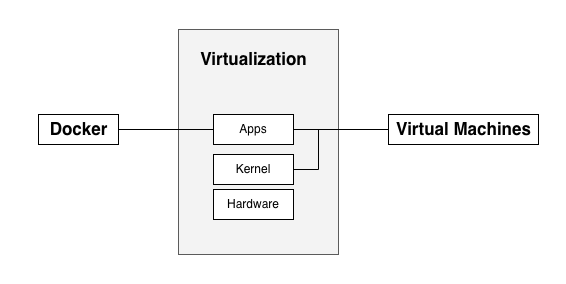
\includegraphics[width=0.5\textwidth]{img/docker-vs-vms.png}
        \caption{Docker vs VMs}
        \label{fig:my_label}
    \end{figure}

    \paragraph{Types of Virtualization} Exists three types of virtualization:
    \begin{itemize}
        \item \textbf{Para-Virtualization}: In para-virtualization, the host is trying to give the guest most of their hardware. 
        \item \textbf{Partial Virtualization}: Where some components of the host's hardware are virtualized and given to the guest.
        \item \textbf{Full Virtualization}: In full virtualization, the guest is given a full copy of the host's hardware.
    \end{itemize}

    For each of this cases, Docker is going to be superior, as Docker uses the kernel of the host directly.

    \subsection{Docker Network}

    \paragraph{Network} A Network in simple terms is a group of two or more devices that can communicate with each other either physically or virtually.

    \paragraph*{Docker Network} The Docker Network  is a virtual network created by Docker to enable communication between Docker Containers. Container Networking refers to the ability for containers to connect to and communicate withe ach other, or to non-Docker workloads.

    Containers have networking enabled by default, and they can make outgoing connections. A container has no information about what kind of network it's attached to, or whether their peers are also Docker workloads or not. 

    \paragraph*{Port Mapping} is a way to allow traffic to flow from the outside world into a container. Since containers are isolated environments, if you want to access a web application inside a container from your web browser, you need to map the port on which the application is running inside the container to a port on the host machine.

    \begin{figure}[h]
        \centering
        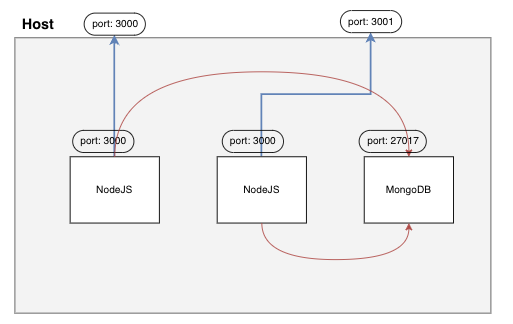
\includegraphics[width=0.5\textwidth]{img/docker-port-mapping.png}
        \caption{Docker Port Mapping}
        \label{fig:docker-port-mapping}
    \end{figure}

    As per the figure above, the Node JS container is running on port 3000. To access this container from the host machine, we need to map the port 3000 of the container to a port on the host machine. In this case, we're mapping the port 3000 of the container to the port 3000 of the host machine. 

    Usually, you would find that in cases where you have multiple containers running on the same port, you would map the port of the container to a different port on the host machine. So, if you have two containers with Node JS each with a web application running on port 3000, you would map the port of the first container to port 3000 of the host machine, and the port of the second container to port 3001 of the host machine. Although this is not mandatory, it's a good practice to avoid conflicts.




    \subsection{}
    \subsection{}
    
    \newpage
    \section{Amazon Web Services}
    \subsection{}
    \subsection{}
    
    \newpage
    \section{Terraform}
    \subsection{}
    \subsection{}
    
    \newpage
    \section{Ansible}
    \subsection{}
    \subsection{}

    \newpage
    \section{Github Actions}
    \subsection{}
    \subsection{}



\end{document}

    % Stick Notes examples 
    % % Put the sticky note in a wrapfigure to have text wrap around it.
    % \begin{wrapfigure}{L}{0.45\textwidth}
    %     \begin{YStkyNote}[Note 1]
    %         This text is \emph{important}. Here is an useful equation:
    %         \begin{align}
    %             \sin (x) \approx x
    %         \end{align}
    %     \end{YStkyNote}
    % \end{wrapfigure}

    % \begin{wrapfigure}{R}{0.45\textwidth}
    %     \begin{PStkyNote}[Note 2]
    %     Here is some more text. This is useful information you need to know:
    %     \begin{itemize}
    %         \item sin approximation valid \textbf{only} for small angles
    %         \item 2 radians is \textit{not} a small angle
    %     \end{itemize}
    %     \end{PStkyNote}
    % \end{wrapfigure}

    % \begin{wrapfigure}{L}{0.45\textwidth}
    %     \begin{GStkyNote}[Note 3]
    %     \NB do not forget this!
    %     \end{GStkyNote}
    % \end{wrapfigure}

    % \begin{wrapfigure}{R}{0.45\textwidth}
    %     \begin{BStkyNote}[Note 4]
    %     This will be on the final exam!
    %     You better \emph{study} hard!
    %     \end{BStkyNote}
    % \end{wrapfigure}

    % \begin{wrapfigure}{L}{0.45\textwidth}
    %     \begin{WStkyNote}[Note 5]
    %         \begin{equation}
    %             pV=Nk_BT
    %         \end{equation}
    %     \end{WStkyNote}
    % \end{wrapfigure}

    % \begin{wrapfigure}{R}{0.45\textwidth}
    %     \begin{BrStkyNote}[Note 6]
    %     Type \verb+\NB+ to get the \NB text.
    %     \end{BrStkyNote}
    % \end{wrapfigure}